\documentclass[14pt]{extarticle}
\usepackage[utf8]{inputenc}
\usepackage[T1]{fontenc}
\usepackage[french]{babel}
\usepackage{csquotes}
\usepackage[backend=biber,style=numeric,sorting=none,backref,natbib,hyperref]{biblatex}
\usepackage{graphicx}
\usepackage{amsmath}
\usepackage[colorlinks=true]{hyperref}
\usepackage[indent=40pt]{parskip}
\usepackage{indentfirst}
\usepackage{enumitem}
\usepackage{comment}

\addbibresource{ref.bib}
\nocite{*}


\begin{document}

%première page
\begin{titlepage}
    \begin{center}
        
\includegraphics[width=0.4\textwidth]{img/su.png}
        \hspace{4cm}
        
\includegraphics[width=0.2\textwidth]{img/LIP6.png}

        {\Large \textbf{\\Sciences Informatiques\\}
        \textit{\\RAPPORT\\}}
        \vspace{0.2cm}
        {\large \text{Été 2023}}

        \vfill
       
        {\Large \textbf{Répartition statique et dynamique de machines virtuelles sur cluster Proxmox\\}}

        \vspace{1cm}
       
        \textbf{Maxime Derri\\}
        Encadré par Françis Hulin-Hubard et Julien Sopena\\

       \vfill
    \end{center}
\end{titlepage}



%table des matières
\hypersetup{
    linkcolor=blue,
    filecolor=magenta,      
    urlcolor=cyan,
    pdftitle={proxmox-placement},
}
\urlstyle{same}
\tableofcontents
\newpage



\section*{Introduction}
    \addcontentsline{toc}{section}{Introduction}
    Ces dernières années, l'avancée technologique à permit de produire des composants matériels de meilleur qualitée. Les entreprises sont en mesure de produire des machines comprenant des processeurs composés de dizaines de coeurs accompagnés d'une grande quantitée de mémoire ainsi que plusieurs teraoctets d'espace disque.\\
    L'essor de la virtualisation à permit de créer des infrastructures dont la maintenance et la surveillance sont simplifiées grace aux différentes composantes matérielles et logicielles.\\
    Les serveurs physiques (noeuds) étant de plus en plus performants, leur nombre s'en voit condensé.\\
    De plus, il est possible de mettre en place des liens entre ces noeuds afin de les rassembler sous un cluster dont l'objectif est de simplifier la gestion des infrastructures.\\
    \\
    Nous allons nous intéresser à l'un des outils de la virtualisation, la migration.\\
    La migration est le fait de déplacer un conteneur (CT) ou une machine virtuelle (VM) d'un noeud à un autre.\\
    L'objectif de ce travail est de mettre en place un utilitaire permettant de réordonner les conteneurs et les machines virtuelles sur un cluster Proxmox.\\
    Un tel outil aura pour mission d'équilibrer l'utilisation des ressources matérielles d'un cluster et de vider un noeud afin de l'éteindre pour une maintenance.\\
    Nous prendrons appuis sur Proxmox qui est une solution de virtualisation libre.
    \newpage
    
    \noindent
    Au travers de ce document, nous parlerons de Proxmox et de son fonctionnement.\\
    Puis, nous parlerons de l'architecture générale de l'outil.
    Enfin, nous détaillerons en plusieurs sections les étapes effectuées par l'utilitaire dont le fonctionnement se rapproche d'une boucle MAPE-K.
    \newpage



\section{Proxmox: une solution de virtualisation libre de droit}
    \subsection{Généralitées sur les systèmes de virtualisation et présentation de Proxmox}
    La virtualisation consiste à exécuter sur une machine, dans un environement isolé, plusieurs systèmes d'exploitation. Cela permet de rassembler sous une même machine plusieurs machines virtuelles qui peuvent fournir des services comme l'exécution de serveurs au sens logiciel. Un environnement virtuel permet donc de réduire le nombre de machines physiques (maintenance simplifiée), de réduire la consommation d'énergie ainsi que de réduire les coûts.\\
    De plus, il est généralement possible de réaliser un cluster (aussi appelé grappe de serveurs) en mettant en relation plusieurs noeuds afin qu'ils puissent s'échanger des informations sous un même protocol. Cela permet la migration des machines virtuelles et des conteneurs, c'est à dire le déplacement d'un noeud à un autre. Cette fonctionnalité peut être utilisée afin d'équilibrer les charges et de vider des noeuds d'un cluster.\\
    \\
    Proxmox \cite{pve} est un ensemble logiciel sous licence AGPL permettant de mettre en place la virtualisation. Il supporte l'exécution des machines virtuelles Qemu, des conteneurs LXC et fournit des utilitaires ainsi qu'un ISO à installer.\\
    Les clusteurs sont basés sur Corosync Cluster Engine, un projet open source écrit en C. Les utilitaires de Proxmox sont par contre écris en Perl et l'interface web en JavaScript.
    \newpage
    \begin{figure}[!h]
       \centering
        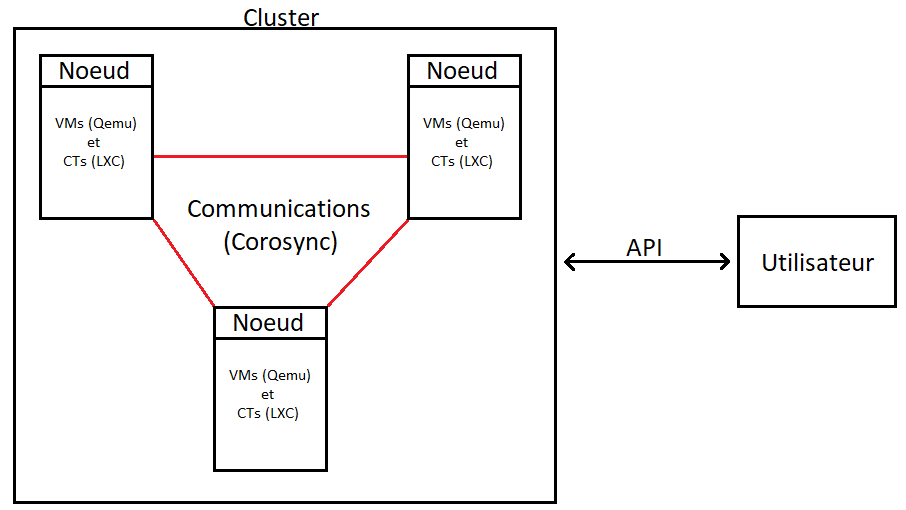
\includegraphics[width=1\textwidth]{img/cluster.png}
        \label{Schéma d'un cluster Proxmox}
        \caption{Schéma d'un cluster Proxmox}
    \end{figure}
    \noindent
    Sous Proxmox, il existe deux types de migration:
    \begin{itemize}[nosep,label=\textendash]
        \item Offline migration, la VM ou le CT n'est pas allumé, il faudra copier son contenu sur la cible et nettoyer la source.
        \item Live migration, uniquement pour les VMs en cours de fonctionnement. Permet de migrer la VM sans interruption de service.
    \end{itemize}
    Aussi, Proxmox offre plusieurs types de stockage:
    \begin{itemize}[nosep,label=\textendash]
        \item Local, comme ZFS, LVM thin, répertoires, etc... Le contenu est disponible uniquement sur la source.
        \item Partagé, comme NFS, etc... Le contenu est stocké sur une machine, mais est accessible à travers le réseau. 
    \end{itemize}
    Donc une VM dont l'image est stockée sur un stockage partagé sera plus rapide à migrer.\\
    On pourra migrer uniquement l'état de la VM et l'opération sera terminée.\\
    \\
    Pour communiquer avec les noeuds, Proxmox définit une API \cite{api} dont les échanges se font sous le format des fichiers JSON. Il est possible de faire des utilitaires car les outils fournis avec Proxmox utilisent généralement cette API. On est donc en mesure de récupérer des informations sur le cluster, sur les noeuds, sur les VMs et les CTs, créer des stockages ou en supprimer, effectuer des migrations, etc...\\
    \\
    Enfin, dans un soucis de simplification, une interface utilisateur web est disponible afin de gérer graphiquement les noeuds. La plupart des fonctionnalités y sont accessibles, mais certaines opérations demandent de passer par un terminal.
    \newpage


    \subsection{Fonctionnement des migrations sur Proxmox}
    Dans cette sous-section, nous allons expliquer comment Proxmox effectue les migrations en prenant appuis sur le cas des machines virtuelles du projet Qemu. Il faut noter que Qemu fournit dans ses sources des outils pour la migration.\\
    Expliquer la migration des conteneurs LXC serait redondant. De plus, les conteneurs peuvent être migrés uniquement s'ils ne sont pas démarrés.\\
    \\
    Il existe plusieurs façons de déclancher une migration. On peut passer par l'interface web ou les utilitaires en ligne de commande en utilisant un wrapper de l'API.\\
    Cependant, toute demande est reçue par le noeud possédant actuellement la VM car l'API à besoin du nom du noeud source, de la cible et de l'identifiant de la VM. Lors d'une migration, si la VM possède des données locales alors il va falloir faire un choix sur les stockages du noeud cible.\\
    Il existe 3 possibilités:
    \begin{itemize}[nosep,label=\textendash]
        \item Ne rien sélectionner. Dans ce cas, Proxmox va essayer de faire correspondre le nom des stockages de la source et de la cible. Si un nom n'existe pas, alors la migration échouera.
        \item Sélectionner une seul cible. Ici, Proxmox va essayer d'envoyer les images sur ce stockage. Il est également possible que la migration échoue pour des problèmes de compatibilité de format et/ou de type de stockage.
        \item Sélectionner plusieurs stockages. Le format est le suivant:\\
        \shorthandoff{:}\textbf{src1:tgt1[,;]src2:tgt2[,;]...srcN:tgtN}\shorthandon{:}.\\
        Ainsi, on peut transférer les images d'un stockage à un autre sans contrainte sur les noms.
    \end{itemize}
    Il existe des différences entre le passage par l'interface web et les utilitaires, que ce soit des programmes venant du projet Proxmox ou non. En effet, l'interface web n'implémente pas la sélection de plusieurs stockages sur la cible.\\
    \\
    Premièrement, quand une demande de migration est reçue par un noeud, celui-ci va extraire les informations reçues au format JSON afin de vérifier les attributs. C'est également à ce moment là que les stockages du noeud source et cible seront étudiés.\\
    Deuxièmement, la VM sera verouillée par un fichier que Proxmox aura généré (/var/lock/pve-manager/pve-migrate-\$vmid).\\
    Troisièmement, l'étape de la migration va commencer en verouillant un fichier de configuration (/var/lock/qemu-server/lock-\$vmid.conf) et en faisant des vérifications sur l'état des noeuds, de la VM, des stockages, des taches démarrées par Proxmox, etc...\\
    L'étape de la migration est séparée en trois parties:
    \begin{itemize}[nosep,label=\textendash]
        \item La \underline{phase1}. Le fichier de configuration de la VM sera mis à jour pour bien définir la taille des images. Si la réplication est activée, alors une mise à jour des répliques sera faite en mettant à jour une bitmap par le calcul d'un delta (une différence), puis en effectuant le transfère en utilisant le mécanisme de snapshot. Les images hors lignes seront également envoyées depuis cette étape. Cela veut dire qu'une VM éteinte verra toutes ses images migrées.\\
        Dans un premier temps, la connexion est établie et une commande est fournie au noeud cible pour récupérer plus tard le contenu des images.\\
        Dans un deuxième temps, des requêtes sont envoyées à la cible pour qu'elle s'occupe de la création des images au bon format (avec des outils comme \textbf{qemu-img}).\\
        Quand c'est fini, la cible va récupérer le contenu des images.
        \item La \underline{phase2}, qui est réservée à la live migrations.\\
        La VM va être démarrée sur le noeud cible et les images lui seront accessibles sur le réseau par l'utilisation du protocol Network Block Device (NBD).\\
        Ensuite, les images seront migrées par l'utilisation d'une commande \textbf{drive-mirror} du projet Qemu qui utilise NBD.\\
        Vient ensuite la migration de l'état de la VM. Un ensemble de paramètres est renseigné à Qemu, dont un cache xbzrle \cite{xbzrle} utilisé pour les transferts. C'est les sources de Qemu qui vont s'occuper de cette partie.\\
        Qemu fourni du code pour réaliser les migrations en proposant deux méthodes: \textbf{precopy} et \textbf{postcopy} \cite{qemu-migration,post_precopy_schem}.\\
        Pour Proxmox, c'est très probablement la precopy qui est utilisée. Elle fonctionne ainsi:
        \begin{itemize}[nosep,label=\textendash]
            \item Copier tout la mémoire sur la VM du noeud cible.
            \item Copier les pages qui ont été modifiées pendant le précédent transfert. Ce point est relancé tant que le nombre de pages modifiées atteint un plafond.
            \item La VM du noeud source est bloquée.
            \item Les dernières pages modifiées, l'état du CPU et des devices sont envoyés.
            \item La VM du noeud cible prend pleinement la main.
        \end{itemize}
        \item La \underline{phase3}, qui sert pour nettoyer après la migration (comme les images du noeud source).
    \end{itemize}
    \newpage



\section{Architecture générale du projet}
    \subsection{Problème de bin packing}
    Avant de parler du problème de bin packing, il faut introduire quelques explications sur les classes de complexité.\\
    \\
    En algorithmique, on utilise la complexité pour mesurer la performance d'un algorithme. On peut par exemple compter le nombre d'opérations élémentaires (calculs), le nombre d'opérations sur des structures de données ou encore le nombre de messages envoyés. Tout problème ne peut pas être résolu de manière efficace (en temps logarithmique, linéaire ou polynomial). Nous ne pouvons pas nous baser sur le temps car celui-ci va varier en fonction du matériel de la machine utilisée et du système d'exploitation (entrées / sorties, ordonnancement des processus, etc...).\\
    Ainsi, on introduit des classes de complexité.\\
    On appel classe P, la classe des problèmes de décision qui peuvent être résolus par une machine de Turing déterministe en temps polynomial. Plusieurs algorithmes sont dans la classe P comme Dijkstra, DFS, Kruskal, Prime, Quicksort et beaucoup d'autres.\\
    On appel classe NP la classe des problèmes de décision qui peuvent être résolus par un machine de turing non déterministe. On peut donc vérifier en temps polynomial si le résultat d'un algorithme est une solution du problème ou non. Par exemple, le problème du voyageur de commerce, le problème de bin packing, le problème de coloration de graphe et le problème de satisfiabilité sont dans la classe NP.
    \newpage
    \begin{figure}[!h]
        \centering
        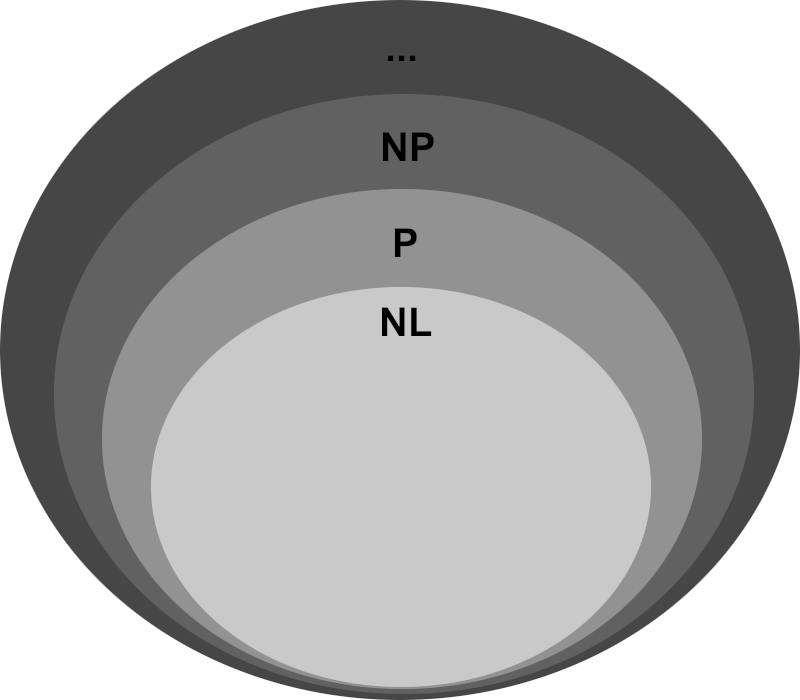
\includegraphics[width=0.7\textwidth]{img/classe_complexite.png}
        \label{Classes de complexité}
        \caption{Classes de complexité}
    \end{figure}
    \noindent
    On appel NP-difficile un problème qui est au moins aussi difficile que les problèmes les plus difficiles de la classe NP. Donc, ces problèmes peuvent ne pas appartenir à la classe NP. De plus, on dit qu'un problème A est NP-difficile si les problèmes B appartenant à NP peuvent être réduits en temps polynomial à A. Cela veut dire que s'il existe un algorithme qui résout A en temps polynomial, alors on peut construire un algorithme qui résout tous les problèmes NP.\\
    Enfin, on appel NP-complet un problème qui est à la fois NP et NP-difficile. Le problème du voyageur de commerce en est un exemple. Il appartient à NP car on peut décider en temps polynomial si un résultat est solution ou non en vérifiant qu'il ne passe pas par une même place plus d'une fois. Il est également NP-difficile car on peut réduire le problème du cycle Hamiltonien à ce problème.\\
    \newpage
    \begin{figure}[!h]
        \centering
        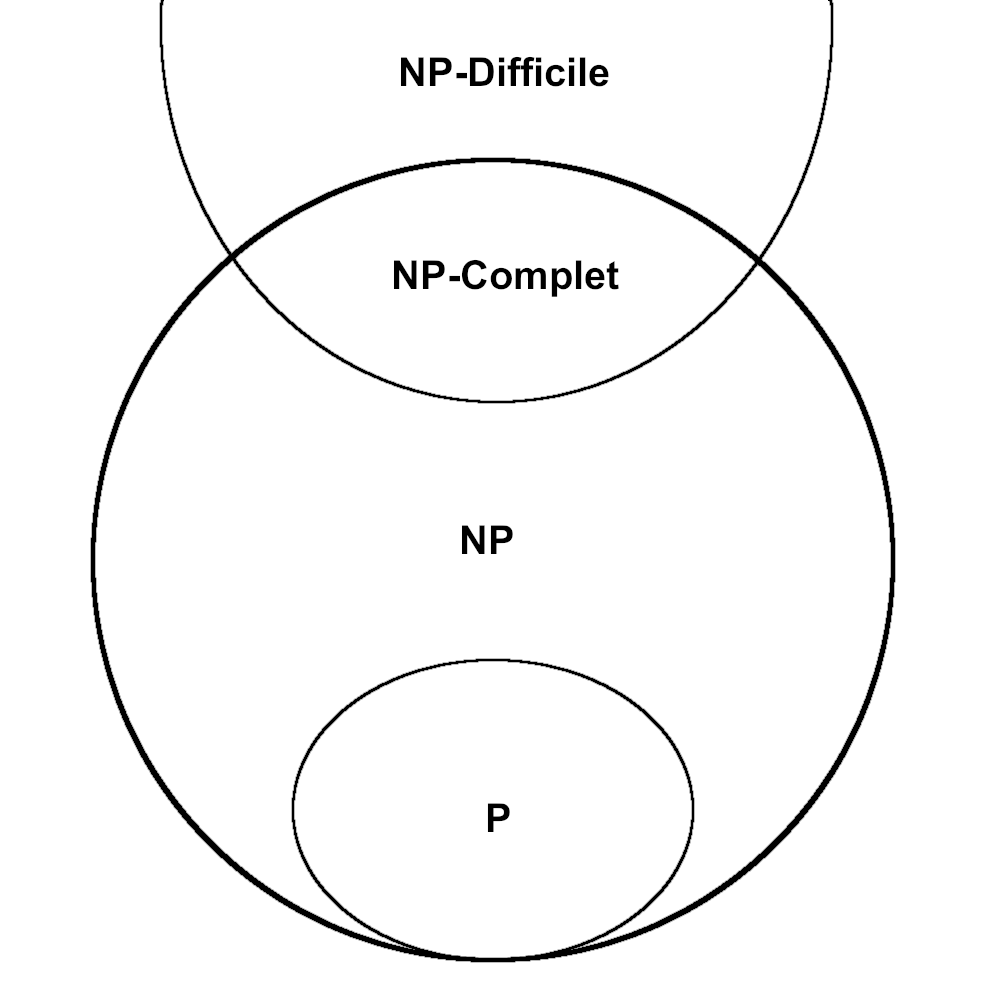
\includegraphics[width=0.7\textwidth]{img/np-complet.png}
        \label{NP-complétude}
        \caption{NP-complétude}
    \end{figure}
    \noindent
    Le problème du bin packing est connu pour être NP-complet.\\
    En effet, il est dans la classe NP car on ne peut pas résoudre ce problème de manière optimale avec une machine de Turing déterministe en temps polynomial. De plus, la vérification du résultat se fait bien en temps polynomial car il faut parcourir les boites et vérifier si le placement est correct.
    Aussi, il est NP-difficile car on peut réduire en temps polynomial le problème de bipartition.\\
    Supposons qu'il existe un certain nombre de boites B et d'objets O. Le problème classique (une dimension) est de ranger tous les objets O dans un nombre minimal de boites B. Le problème peut être étendu en ajoutant des contraintes sur les objets (taille, poids, etc...).\\
    Ainsi, nous pouvons considérer les objets comme des VMs et CTs avec des contraites d'espace disque, RAM, CPU et les boites en tant que noeuds du cluster.\\
    Cela signifie également que les algorithmes de placement des VMs et CTs peuvent être basés sur le problème de bin packing. Comme ce problème est NP-complet, il va être nécessaire de produire des algorithmes d'approxmiation sinon la complexité sera exponentielle. Un algorithme d'approximation fourni un résultat qui se rapproche de la solution optimale (donc résultat non parfait), mais avec une complexité polynomiale.
    \newpage


    \subsection{Boucle MAPE-K}
    Le programme à construire pour ce projet doit permettre de proposer une suite de migrations, si c'est nécessaire, pour réordonner les noeuds d'un cluster.\\
    Il sera nécessaire de récupérer des informations sur le cluster, il faudra ensuite vérifier l'état du cluster pour savoir s'il est nécessaire de proposer une nouvelle organisation, puis l'appliquer en déplaçant les machines virtuelles et les conteneurs entre les noeuds.\\
    La réalisation d'une telle architecture est semblable à celle d'une boucle MAPE-K (Monitorring, Analysis, Planning, Execution, Knowledge). Ce principe décompose un programme en plusieurs étapes qui ont un rôle dans l'exécuction de la boucle.\\
    On retrouve 5 parties:
    \begin{itemize}[nosep,label=\textendash]
        \item Surveillance: Le fait de récupérer des informations sur le système.\\
        Proxmox, à travers son API \cite{api}, nous permet de récupérer des informations sur le fonctionnement du cluster. Cette méthode est relativement simple et accesible car il existe plusieurs wrappers de l'API. Dans notre cas, nous utiliserons Proxmoxer \cite{proxmoxer} qui est écrit en python3.\\
        \item L'analyse: Elle suit l'étape de surveillance car cette dernière utilise les données récupérées.\\
        L'objectif est de déduire un déséquilibre du système afin de décider s'il est nécessaire ou non d'effectuer un équilibrage.\\
        On regardera l'utilisation CPU des noeuds du cluster car une trop grosse charge peut provoquer des ralentissements.\\
        On va aussi s'intéresser à la RAM car il est possible d'allouer plus de RAM que celle disponible sur le noeud. De plus, il faut prendre en compte que le système et les utilitaires ont besoins de RAM pour fonctionner (au moins 2Go). Il sera également nécessaire de compter 1 Go de RAM par To de stockage ZFS.\\
        Enfin, on surveillera l'utilisation des espaces de stockage des noeuds car un stockage trop rempli peut ralentir le système.
        \item La planification: trouver une solution au déséquilibre.\\
        Ici, c'est notre algorithme basé sur le problème de bin packing qui sera appelé. Il produira en sortie une liste d'action à effectuer avant la migration (si nécessaire), ainsi que la liste ordonnée des migrations à effectuer pour tenter d'améliorer la situation du cluster.
        \item L'exécution: l'étape qui corrige le problème.\\
        Cette partie à pour but d'utiliser le résultat de l'algorithme afin de guider le script qui effectue les migrations une par une. L'API de Proxmox fourni des commandes pour lancer ces migrations.
        \item Knowledge: représente le système et la prise de décisions.\\
        Dans l'étape knowledge, il sera question dans un premier temps de la représentation du cluster. Cela sera fait par le côté orienté objet de python qui permet de décrire les éléments du cluster sous des objets.\\
        Dans un deuxième temps, il sera question du lancement de la boucle des étapes. On peut soit décider de la lancer de notre plein gré, soit utiliser une fonctionnalité de l'utilitaire qui fera une ronde d'analyse à interval régulier. 
        Cette dernière proposition se base sur la lecture (avec SSH sur chaque noeud) du fichier /proc/pressure/cpu \cite{kernel_psi} qui donne un indice en fonction des taches bloquées sur des ressources.
    \end{itemize}
    \newpage



\section{Surveillance du système}
    \subsection{Les outils de surveillance}
    La récupération d'informations sur le système est une étape très importante car les analyses et les plannifications seront basées sur l'extraction de ces données. Tous les utilitaires de Proxmox passent par son API. Cette architecture permet aux développeurs de créer des logiciels tiers. On peut y récupérer de nombreuses informations sur les noeuds comme le type de CPU utilisé par un noeud, les flags CPU d'un noeud, les interfaces réseaux liées à un noeud, etc...  Ces informations seront utiles car avant de planifier une migration, il faut savoir si la machine virtuelle ou le conteneur peut être hébergé par un autre noeud.\\
    L'API de proxmox met aussi à disposition des requêtes qui permettent de récupérer des échantillons d'utilisation CPU et RAM sur différentes périodes. Cette fonctionnalité est très pratique pour réaliser des moyennes d'utilisation car une machine virtuelle ou un conteneur pourrait très bien fonctionner à pleine charge sur une très courte période et notre système pourrait considérer cela comme un déséquilibre alors que cet évenement est assez rare.\\
    Il faut cependant noter que les échantillons des charges CPU reçues par l'API mesurent l'utilisation des ressources allouées à un noeud, et non pas de la machine physique. Nous y reviendrons dans la prochaine sous-section.\\
    \\
    D'autres informations peuvent aussi être récupérées au travers d'échanges avec SSH. Cependant il sera nécessaire de programmer nos sondes.\\
    On peut y extraire des informations de la commande TOP, ce qui donne des informations sur l'utilisation des ressources de la machine physique et plus uniquement du noeud Proxmox. Il faut cependant faire attention car l'affichage de l'utilisation CPU d'un noeud Proxmox n'est pas forcément la même que celle résultant de l'affichage de la commande TOP. Par exemple sur un cluster de test, nous avons déjà eu un noeud Proxmox avec le CPU à 100\%, alors que la commande TOP nous affichait environ 50\% d'utilisation.\\
    D'autres éléments pourraient aussi être récupérés sur les systèmes Linux comme la pression  exercée sur le système (/proc/pressure/) \cite{kernel_psi} ou bien des informations sur le CPU (/proc/cpuinfo).\\
    \\
    On ne peut pas se baser sur toutes les informations car cela va allourdir le code et amplifier la complexité des algorithmes. Pour cela, nous utiliserons en grande partie les données issues de sondes CPUs, RAMs et disques.
    \newpage


    \subsection{Mesurer l'utilisation des ressources CPU des machines virtuelles et des conteneurs}
    En passant par l'API de Proxmox, il est possible de récupérer la part des ressources qui sont utilisées sur les ressources allouées des machines virtuelles et des conteneurs. A partir de ces valeurs, Proxmox déduit la part des ressources utilisées par les machines virtuelles et les conteneurs sur les ressources du noeud avec le calcul suivant:\\
    Notons L l'utilisation CPU de la VM ou du CT, N le nombre de coeurs du noeud et V le nombre de coeurs alloués à la VM ou au CT.\\
    Proxmox utilise la formule suivante: L / N * V.\\
    Ce calcul ne prend pas en compte l'utilisation CPU du noeud ou de la machine physique pour donner la part des ressources utilisées. On va chercher à le prendre en compte.\\
    \\
    Soit $L_i$ l'utilisation du CPU de la VM ou du CT i et $C_i$ le nombre de coeurs associés à $M_i$.\\
    Notons $T = \sum_{i = 0}^j L_i * M_i$, la somme des charges des machines virtuelles et conteneurs.\\
    Enfin, C désigne la charge CPU du noeud ou de la machine physique.\\
    Si on considère utiliser une architecture hétérogène, alors on peut laisser de côter la part des ressources utilisées par le système et les utilitaires et considérer uniquement les machines virtuelles et les conteneurs. Pour l'algorithme, nous allons considérer que la part des ressources utilisées par une machine virtuelle ou un conteneur sur les ressources de son noeud est obtenue par $C * \frac{L_i * M_i}{T}$.\\
    \newpage
    \noindent
    nous allons énumérer deux possibilitées en fonction de C:
    \begin{itemize}[nosep,label=\textendash]
        \item C désigne la charge CPU calculée de la machine physique ou encore sa load average \cite{load_average}.\\
        L'avantage est que nous allons considérer les ressources utilisées sur le serveur car le noeud est le serveur. De cette façon, on pourra déduire une utilisation approximative d'une VM ou d'un CT sur les ressources du serveur.\\
        Cependant, comme expliqué dans la sous-section 3.1, l'utilisation CPU affichée par TOP et par Proxmox sont différentes. Si on considère uniquement l'utilisation CPU donnée par le système, on peut se retrouver dans une situation où on ne pourrait pas définir une ligne rouge d'utilisation CPU. Si Proxmox est à 100\%, le système pourrait retourner une valeur différente d'une architecture à l'autre.\\
        Aussi, cela pourrait mener à surcharger un noeud si son système indique une utilisation faible ou moyenne mais que Proxmox est en surcharge, et que l'on y migre plusieurs VMs ou CTs.\\
        Enfin, il pourrait être nécessaire de programmer une sonde qui récupère périodiquement des échantillons d'utilisation CPU pour faire des moyennes. Cette outil pourrait consommer des ressources.
        \item C désigne l'utilisation CPU du noeud retournée par l'API de Proxmox.
        L'avatange est que l'on est en mesure de poser une ligne rouge d'utilisation CPU et il n'y aura pas de variation entre système et Proxmox comme expliqué dans le point précédent.\\
        Aussi, une sonde est disponible en passant par l'API. Elle permet de récupérer des échantillons d'utilisation CPU et RAM sur une période que l'on peut préciser.\\
        Cependant, Plus la période est étendue, plus les échantillons retournés sont distants dans le temps. Il faut prendre en compte que les échantillons sont stockés et qu'en accumuler en trop grande quantitée risque de nécessiter trop de mémoire et de stockage.
    \end{itemize}
    Pour ce travail, il a été décidé d'utiliser la valeur retournée par Proxmox. L'utilisation du CPU de la machine physique est une autre piste qui nécessiterait plus de temps pour faire des tests, pour proposer une plateforme afin de récupérer des échantillons pour faire des moyennes ainsi que pour décider d'une méthode pour désigner une ligne rouge d'utilisation CPU.
    \newpage



\section{L'analyse et la planifier des migrations}
    Cette section va traiter deux parties de la boucle MAPE-K, l'analyse et la planification.\\
    Ces deux parties seront discutées en même temps car les analyses sont effectuées pendant l'algorithme.\\

    \subsection{Algorithmes de placement}
    Comme vue précédemment, notre problème de placement se rapproche du problème de bin packing. Il existe plusieurs méthodes pour résoudre ce problème mais nous allons nous intéresser à deux algorithmes: Le First-Fit et le Best-Fit.\\
    \\
    Le First-Fit et le Best-Fit possèdent des similitudes sur leur fonctionnement: On va chercher une boite pour y ranger notre objet. Si on n'en trouve pas, alors on ajoute une nouvelle boite et on continue. Ces deux algorithmes se différencient principalement sur la façon de sélectionner la boite.\\
    Le First-Fit va chercher la première boite qui correspond et va s'en servir pour y ranger l'objet. S'il ne trouve pas de boite convenable, il ajoute une nouvelle boite et y range l'objet.\\
    Le Best-Fit va parcourir toutes les boites et garder uniquement celle qui correspond le mieux. Si aucune ne correspond, une nouvelle boite contenant l'objet est ajoutée.
    \newpage
    \begin{figure}[!h]
        \centering
        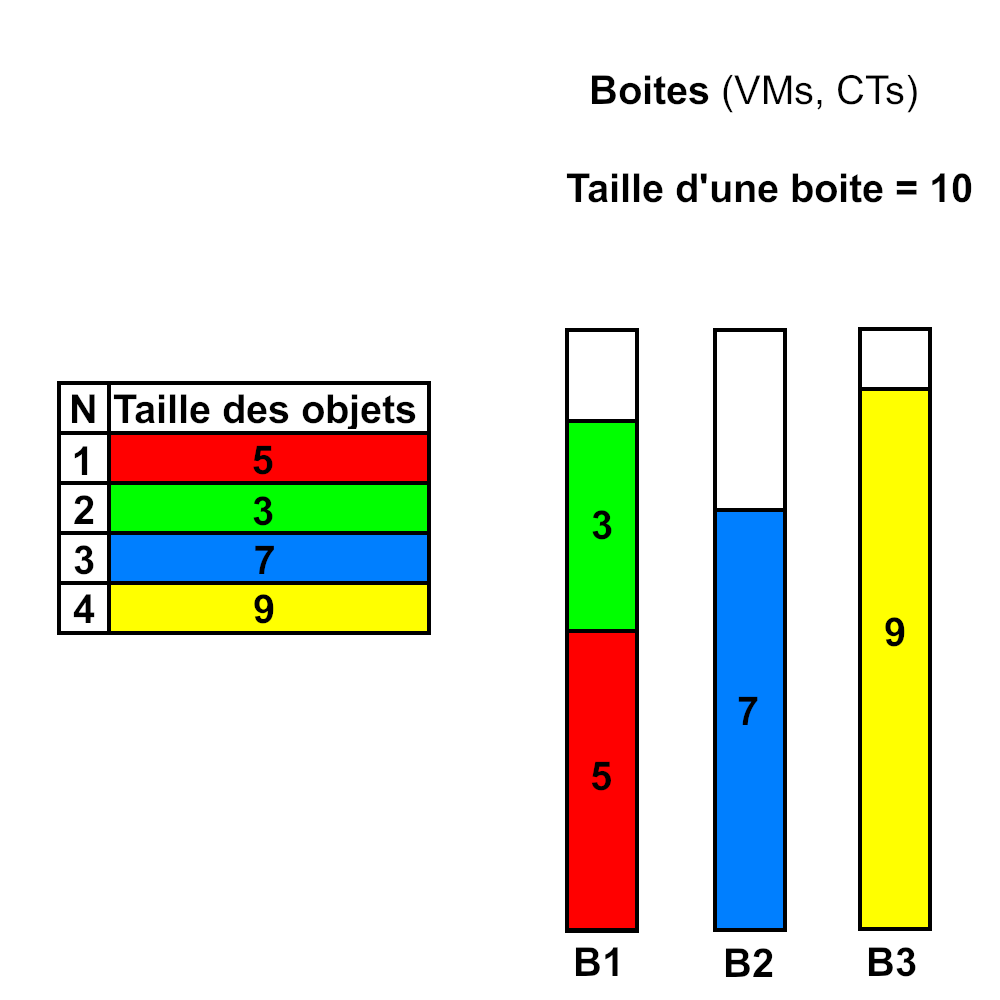
\includegraphics[width=0.8\textwidth]{img/bin_packing.png}
        \label{Problème de bin packing et rangement}
        \caption{Problème de bin packing et rangement}
    \end{figure}
    \noindent
    Il existe également des variantes où un pré-traitement est effectué au début de l'exécution.\\
    Par exemple, il est possible de trier la liste des objets par ordre décroissant en fonction de leurs caractéristiques. C'est ainsi que fonctionne le First-Fit decreasing et le Best-Fit decreasing. On va chercher à placer en premier les objets les plus encombrants et on complète avec les plus petits.\\
    \\
    Les solutions générées par l'un ne sont pas nécessairement meilleures que celles générées par l'autre car les deux donneront des résultats différents du fait que l'on utilise des algorithmes d'approximation.\\
    Aussi, comme dit, il existe d'autres méthodes de résolution du problème de bin packing \cite{bin_pack_wiki_algos}\\
    \\
    Pour réaliser l'implémentation d'un algorithme de placement de machines virtuelles et de conteneurs, il faut adapter ces solutions en prennant en compte les contraintes logicielles que l'on s'est fixé et celles de la solution de virtualisation:
    \begin{itemize}[nosep,label=\textendash]
        \item On ne peut pas ajouter de boites car elles correspondent aux noeuds du cluster.
        \item Il faut faire attention au nombre de migrations car un certain temps est requis pour compléter le processus. De plus, cela consomme des ressources.
        \item Il faut instaurer un ordre d'exécution des migrations car on pourrait se retrouver en manque d'espace si une migration précédente censée libérer de l'espace disque nécessaire n'a pas été effectuée.
        \item On doit prendre en compte que les migrations peuvent nécessiter de créer des stockages sur des noeuds cibles si jamais on considère qu'un stockage dépasse ou peut dépasser une limite \cite{linux_perf_fs}, ou bien qu'une VM doit être déplacée pour réduire la charge de son noeud source et qu'un type de stockage n'est pas disponible sur la cible.
        \item ZFS et lvmthin se basent sur un pool de données qui peut être partagé entre plusieurs stockages de même type sur un même noeud. Il faut faire attention à l'identification de la place disponible sur ces types de stockage.
    \end{itemize}
    \newpage


    \subsection{Algorithme de placement de machines virtuelles et de conteneurs sur cluster Proxmox}
    Dans cette sous section, nous allons discuter de l'algorithme implémenté.\\
    Le choix de l'algorithme de placement s'est tourné vers le Best-Fit decreasing car plusieurs facteurs sont à prendre en compte au moment de sélectionner des noeuds à chaque itération de la boucle principale.\\
    \\
    Dans le problème de bin packing, les algorithmes commencent avec des boites vides.\\
    Cependant, dans notre cas les noeuds ne sont pas initialement vides. Donc en fonction de l'état du cluster, il se pourrait qu'une machine virtuelle ou un conteneur ne soit déplacé qu'a la fin de l'algorithme. Ce déplacement pourrait débloquer la situation pour effectuer d'autres migrations. Une liste de "dernière chance" a été ajoutée dans le code de l'algorithme afin de relancer la boucle principale dans le cas où au moins une migration a été planifiée. L'algorithme effectuera sa boucle principale au maximum deux fois (une fois si aucune migration n'a été planifiée).\\
    En allant dans ce sens, une ouverture au projet serait d'ajouter à la configuration le choix du nombre d'itération maximum pour essayer de raffiner la solution des itérations précédentes.\\
    Il est aussi à noter qu'une machine virtuelle ou un conteneur planifié pour une migration ne peut pas être resélectionné par cet algorithme.\\
    \\
    Chaque exécution de la boucle principale est précédée par le tri des listes des machines virtuelles et des conteneurs de chacun des noeuds selon leur utilisation CPU. Ces derniers sont stockés dans un dictionnaire dont la clef est le nom du noeud et la valeur est la liste. Ensuite, la boucle principale se lance.\\
    En premier, on va chercher à sélectionner un noeud source. Deux sélections sont faites avant de prendre la décision: on prend le noeud qui consomme le plus de ses ressources CPU et on prend un noeud, s'il existe, dont la RAM allouée (aux VMs et CTs) et nécessaire (utilitaires et ZFS) dépasse sa limite de RAM disponible.
    La sélection est faite comme suit:
    \begin{itemize}[nosep,label=\textendash]
        \item si l'utilisation CPU du noeud sélectionné pour la partie CPU dépasse 80\%, alors ce sera le noeud source.
        \item Sinon, si on a trouvé un noeud qui satisfait le critère de la RAM, alors il sera considéré comme noeud source.
        \item Sinon, si la décision n'a pas été prise et que la configuration impose de migrer toutes les VMs et CTs, alors on sélectionne le noeud du critère CPU.
        \item Sinon, on termine l'algorithme car aucune source ne correspond aux critères et le cluster est considéré comme équilibré.
    \end{itemize}
    On extrait la VM ou le CT en première place de la liste de ce noeud.\\
    Ensuite, on va sélectionner un noeud cible. Comme l'algorithme est basé sur un Best-Fit decreasing, on va parcourir les noeuds et sélectionner celui qui correspond le plus aux critères.\\
    Chaque noeud est d'abord inspecté:
    \begin{itemize}[nosep,label=\textendash]
        \item Pour savoir s'il y a de la place pour la RAM et le CPU.
        \item Si la machine à migrer est une VM et qu'elle n'est pas en fonctionnement, alors on vérifie si la potentielle cible peut héberger cette machine (préconditions de l'API Proxmox).
    \end{itemize}
    Puis, on vérifie:
    \begin{itemize}[nosep,label=\textendash]
        \item Si le CPU de la machine + le CPU du noeud est plus petit ou égal à 80\%, alors:
        \begin{itemize}[nosep,label=\textendash]
            \item Si c'est le premier noeud visité ou que le noeud mit de côté a un CPU supérieur à 80\%, alors on retient ce noeud.
            \item Sinon, si ce noeud nécessite de créer moins (ou pas du tout) d'espace de stockage supplémentaire que le noeud mit de côté, alors on le retient. Il est compliqué de créer des stockages par l'API car il peut être nécessaire de monter un système de fichier et en fonction du type de stockage, il peut être nécessaire de créer un pool de données.\\
            Aussi, on se permet d'accepter un score CPU plus élevé que l'ancien noeud mit de côté car on reste en dessous de la limite des 80\% fixée.
        \end{itemize}
        Dans les deux sous-cas du dessus, si jamais toutes les machines doivent être migrées et que le noeud cible potentiel est le noeud source, alors on passe à l'itération suivante.
        \item Sinon:
        \begin{itemize}[nosep,label=\textendash]
            \item Si c'est le premier noeud sélectionné, que le noeud source est au maximum des capacités de son CPU ou de sa RAM et que la migration n'est pas obligatoire ou que la migration est obligatoire et que le noeud source et cible sont différents, alors on met le noeud de côté.\\
            On fait une distinction sur le fait de devoir migrer toutes les VMs et CTs ou non car migrer du noeud source au noeud cible (qui est aussi la source) revient à ne pas migrer et qu'il est nécessaire de pouvoir gérer cette demande dans ce else.
            \item Sinon, si le CPU du noeud mit de côté est plus grand que le CPU du noeud visité pendant l'itération, alors on le remplace.\\
            Cependant, comme dans les deux sous-cas du if, si jamais la migration est obligatoire et que la source égale la cible, alors on passe à l'itération suivante et on ne sélectionne pas le noeud.\\
        \end{itemize}
        Dans le cas où toutes les machines doivent être migrées, s'il existe au moins un noeud correspondant au if et qu'il est différent du noeud source, alors il sera sélectionné. Sinon, le premier sous-cas du else sélectionnera la cible. Il est bien entendu nécessaire d'avoir au moins deux noeuds dans le cluster.\\
        Il est possible d'avoir le noeud source qui est lui même la cible dans le cas où la migration n'est pas obligatoire. Cela est moins contraignant car dans ce cas on ne prépare pas de migration.\\
        \\
        Lorsqu'une migration est décidée, on ajoute un objet contenant toutes les informations nécessaires dans une liste. Cette liste sera couplée à la fin à une autre liste décrivant les stockages qui doivent être crées à la main. S'il n'y en a pas, alors cette liste est vide.\\
        Les listes seront ensuite serialisées dans un fichier JSON pour conserver les informations. Ces dernières seront utilisées pour l'étape des migrations.\\
        \\
        Un autre algorithme existe, il a été renommé obfd (Old Best-Fit decreasing) car il correspond à un algorithme réalisé dans la première partie du stage comme prototype. Plusieurs points ont été revus et modifiés pour écrire le deuxième algorithme discuté dans ce rapport.
    \end{itemize}
    \newpage



\section{Exécution des migrations}
    Comme nous l'avons vu dans la sous-section 1.2, l'API de Proxmox fournit des fonctionnalités pour effectuer les migrations.\\
    Il est nécessaire de fournir à la requête le nom des noeuds en question, l'id de la machine virtuelle ou du conteneur et les stockages pour transférer les images. Dans le cas d'une machine virtuelle, il est possible de la migrer qu'elle soit en fonctionnement ou non et sans interruption de service. Pour les conteneurs, la migration est seulement possible si ce dernier est éteint. Il est possible de spécifier dans la requête que le conteneur doit être éteint et rallumé une fois le processus de migration effectué.\\
    \\
    Une commande de l'outil du projet permet d'effectuer les migrations en lui fournissant un fichier JSON préalablement généré par l'étape de plannification.\\
    L'outil va commencer par vérifier si les stockages réclamés (s'il y en a) ont été créés.\\
    Puis, une grande boucle while sera exécutée. Pour chaque demande de migration, l'attribut \textbf{targetstorage} de la requête va être construit.\\
    Enfin, la migration sera lancée et l'outil va attendre que la migration soit effectuée en questionnant le cluster au travers de l'API qui peut fournir des informations sur l'avancée des taches de Proxmox.
    \newpage



\section{Représentation du système et prise de décisions}
    Dans cette section il sera question de la partie Knowledge de la boucle MAPE-K discutée à la section 1.2.\\
    \\
    La Représentation d'un système est nécessaire au bon fonctionnement d'un programme.\\
    D'une part, il est intéressant de se pencher sur l'organisation du système. Celle-ci peut être construite en séparant les différentes parties du système dans des structures. Il faut construire la représentation au début du programme, avant tout traitement. Pour Proxmox, cela permet de traiter le cas des migrations par un algorithme en modifiant uniquement la représentation avant tout réel changement. Aussi, on peut exploiter cette représentation pour afficher l'état d'un cluster avant et après une proposition de modification sans avoir à demander à Promox des informations.\\
    D'autre part, du point de vue de la performance, il faut prendre en compte que le traitement des requêtes de l'API prend un certain temps. Construire l'état du système permet de ne pas répéter des requêtes. On pense par exemple à la récupération d'informations sur les machines virtuelles et les conteneurs (noeud possédant la machine, échantillons CPU et RAM, images, etc...).\\
    Utiliser un langage orienté objet rend possible la représentation d'un système en séparant par classe les éléments d'un cluster (VMs et CTs, noeuds, stockages).\\
    \\
    La décision d'exécuter la boucle des étapes peut aussi être considérée. La question est de savoir à quel moment relancer la boucle.\\
    La première possibilitée est de le faire manuellement, en utilisant une commande de l'utilitaire.\\
    La deuxième est de le faire de manière autonome. Au dela de l'étape de l'analyse qui, pour le projet, va étudier la représentation du cluster pour décider des migrations, il va falloir ici observer d'autres variations pour décider quand relancer la boucle des étapes.\\
    Une idée est d'observer la pression sur le système. On peut se pencher sur la pression du CPU \cite{kernel_psi} avec le fichier /proc/pressure/cpu. La première ligne avec \textbf{some} donne un indice sur le temps passé par certains processus à être bloqué sur une ressource. On peut donc considérer qu'une valeur élevée nécessite une attention particulière.\\
    En utilisant une commande, il est possible de lancer l'utilitaire dans un mode autonome. Il ira à interval régulier questionner les noeuds par SSH pour obtenir l'indice de pression de /proc/pressure/cpu. S'il considère qu'une valeur est trop élevée, il déclanchera la boucle. Si un plan de migration à été décidé, il sera effectué. Par contre, si des stockages ont été réclamés, il ne pourra pas être appliqué (section 4.2 et 5).
    \newpage



\section*{Conclusion}
    Au cours de ce stage, nous nous sommes intéressé au problème de placement des machines virtuelles et des conteneurs sur cluster Proxmox.\\
    D'une part, il a été nécessaire de prendre en main cette solution de virtualisation pour comprendre son fonctionnement du point de vue de l'utilisateur. Il a également été indispensable de comprendre son fonctionnement interne en explorant l'API et le code des outils fournis pour construire notre programme.\\
    D'autre part, le placement des machines virtuelles et des conteneurs sur les noeuds d'un cluster est lié au problème de bin packing. Ce dernier a été un point majeur du travail. Le problème étant NP-complet, il a fallu faire le choix d'un algorithme d'approximation pour l'étape de plannification des migrations.\\
    En prennant en compte différents éléments, nous avons décidé de baser l'architecture générale du programme sur une boucle MAPE-K. La structure repose sur plusieurs étapes afin de respecter ce principe. La première étape est la récupération des données du système. Vient ensuite la partie sur l'analyse et la plannification des migrations. Puis, l'exécution du plan décidé à l'étape précédente. A cela s'ajoute la méthode de représentation des données du système ainsi que les façons de déclancher la boucle.\\
    Comme le projet utilise une méthode heuristique, il serait intéressant d'étendre le travail avec d'autres catégories d'algorithmes. Notament, les algorithmes de colonies de fourmis et les algorithmes génétiques.
\newpage


\addcontentsline{toc}{section}{Conclusion}

\printbibliography
\end{document}
